\documentclass[12pt,a4paper,notitlepage]{article}
\usepackage[utf8x]{inputenc}
\usepackage[a4paper,textwidth=17cm, top=2cm, bottom=3.5cm]{geometry}
\usepackage{eurosym}
%\usepackage{url}
\usepackage[T1]{fontenc}
\usepackage{ucs}
\usepackage{ngerman} 
\usepackage{setspace}
%\usepackage{fourier}
\usepackage{amssymb,amsmath}
\usepackage{wasysym}
\usepackage{amsthm}
%\usepackage{marvosym}
\usepackage{tabularx}
\usepackage{multicol}
\usepackage{hyperref}
\usepackage{tabularx}
\usepackage[pdftex]{graphicx,color}
\usepackage{todo}
\definecolor{p-green}{rgb}{0.12,0.57,0.11}
\newcommand{\bitem}{\item[--]}
\newcommand{\litem}[2]{\item[#1 --] #2}
\newcommand{\blitem}[3]{\item[#1 --] \texttt{#2} -- #3}
\newcommand{\gfo}{\grqq\ }
\newcommand{\gfu}{\glqq}
\newcommand{\zquote}[2]{\glqq #1\grqq\ (Z.\ #2)}
\newcommand{\pquote}[1]{\glqq #1\grqq}
\newcommand{\nquote}[2]{#1: \glqq #2\grqq}
\newcommand{\nwquote}[3]{#1 -- \emph{#2}: \glqq #3\grqq}
\newcommand{\nwyquote}[4]{#1 -- \emph{#2} (#3): \glqq #4\grqq}
\newcommand{\diff}{\mathrm{d}}
\renewcommand{\abstractname}{}
\definecolor{orange}{rgb}{1,0.6,0}
\definecolor{d-green}{rgb}{0,0.8,0}
\definecolor{pink}{rgb}{1,0,0.6}
\newcommand{\annot}[1]{\textcolor{red}{#1}}
\newcommand{\ecolor}[1]{\textcolor{pink}{#1}}
\newcommand{\aufgabe}[1]{\section*{\setcounter{section}{#1}Aufgabe #1}}
\newcommand{\re}{\text{Re}}
\newcommand{\im}{\text{Im}}
\onehalfspacing
\setlength{\parskip}{8pt plus4pt minus4pt}
\begin{document}
\begin{center}
\Large Hausaufgaben für P1a

\normalsize Online unter \url{http://github.com/jaseg/Hausaufgaben}
\end{center}
\begin{tabularx}{\textwidth}{Xr}
Jan Sebastian Götte (546408), Paul Scheunemann&Abgabe: 111128
\end{tabularx}
\aufgabe{1}
\subsection*{a}
Es kann $v_{0z}=0$ angenommen werden, da die Bahnkurve des Massepunktes in der Ebene liegen muss, die vom Vektor der Anfangsgeschwindigkeit und vom Vektor der Schwerkraft aufgespannt wird. Durch Rotation und Translation des Koordinatensystems lässt sich somit jede derartige Bewegung auf eine Form bringen, in der $v_{0z}=0$ gilt.
\begin{align}
\vec F_g&=-g\vec e_y\\
\vec F_R&=-m\gamma\dot{\vec x}=-m\gamma\vec v\quad\Big|\vec v=\dot{\vec x}\\
\vec a&=\frac{\vec F}{m}=\dot{\vec v}\\
&=\frac{1}{m}\cdot\left(-g\vec e_y-m\gamma\vec v\right)\\
&=-\frac{g}{m}\vec e_y-\gamma\vec v=\dot{\vec v}\\
\frac{g}{m}\vec e_y+\gamma\vec v+\dot{\vec v}&=0\label{inhomo1}
\end{align}
\ref{inhomo1} ist eine inhomogene lineare Differentialgleichung erster Ordnung. Die Lösung erfolgt im Folgenden über das charakteristische Polynom der zugehörigen homogenen DG mittels Variation der Konstanten.
\begin{align}
\gamma\vec v+\dot{\vec v}=0\:&\Rightarrow\:\left\{\begin{matrix}
\gamma v_x+\dot v_x=0\\
\gamma v_y+\dot v_y=0\\
\gamma v_z+\dot v_z=0\\
\end{matrix}\right.\\
P_\text{Ch}:re^{rx}+\gamma e^{rx}&=0\\
\Rightarrow v_i&=c_ie^{-\gamma t}\\
\Rightarrow \vec v&=e^{-\gamma t}\vec c\\
\vec v(t)=e^{-\gamma t}\vec c(t);&\quad\dot{\vec v}=-\gamma e^{-\gamma t}\vec c(t)+\dot{\vec c}(t)e^{-\gamma t}\\
\frac{g}{m}\vec e_y&=-\dot{\vec v}-\gamma\vec v=\underline{\gamma e^{-\gamma t}\vec c(t)}-\dot{\vec c}(t)e^{-\gamma t}\underline{-\gamma e^{-\gamma t}\vec c(t)}\\
\Rightarrow\frac{g}{m}\vec e_y&=-\dot\vec c(t)e^{-\gamma t}\\
\Rightarrow\dot{\vec c}(t)&=-\frac{g}{m}\vec e_ye^{\gamma t}\\
\vec c(t)&=\int-\frac{g}{m}\vec e_ye^{\gamma t}\diff t\\
&=-\frac{g}{\gamma m}\vec e_ye^{\gamma t}+\vec q\\
\vec v&=e^{-\gamma t}\vec c(t)\\
&=\left(\begin{matrix}
q_1e^{-\gamma t}\\
-\frac{g}{\gamma m}+q_2e^{-\gamma t}\\
q_3e^{-\gamma t}
\end{matrix}\right)\\
\dot{\vec v}&=\left(\begin{matrix}
-\gamma q_1e^{-\gamma t}\\
-\gamma q_2e^{-\gamma t}\\
-\gamma q_3e^{-\gamma t}
\end{matrix}\right)=-\gamma e^{-\gamma t}\vec q\\
\vec x&=\sum\vec e_i\int\dot x_i\diff t\\
&=\vec x_0-\frac{1}{\gamma}\left(\begin{matrix}
q_1e^{-\gamma t}\\
\frac{g}{m}t+q_2e^{-\gamma t}\\
q_3e^{-\gamma t}
\end{matrix}\right)\\
\left(\begin{matrix}
q_1\\q_2\\q_3
\end{matrix}\right)&=\vec v_0
\end{align}
\subsection*{b}
...da sie länger fliegen und somit zur Abschätzung der Flugkurve mehr Zeit verbleibt.
\aufgabe{2}
\subsection*{a)}
\begin{align}
L&=mr_0v_0\\
E&=T+V\\
T&=\frac{1}{2}mv_0^2
\end{align}
Zur Berechnung der potentiellen Energie $V$ muss zunächst die Lage des Equilibriums zwischen Zentrifugalkraft und Schwerkraft bestimmt werden. Doch zunächst ist festzustellen:
\begin{equation}
\dot{\vec L}=\vec 0
\end{equation}
Dies gilt, da die einzige wirkende Kraft radial ist, und dank ihrer Konstanz ein konservatives Kraftfeld bildet. Nun:
\begin{align}
\left|\vec L\right|&=mrv=mr_0v_0\\
\Rightarrow v(r)&=v_0\frac{r_0}{r}\\
F_Z&=-F_R\quad\text{per Voraussetzung}\\
=-m\frac{v(r_t)^2}{r_t}&=-Mg\\
=-m\frac{r_0^2v_0^2}{r_t^3}\\
\Rightarrow r_t&=\sqrt[3]{\frac{mr_0^2v_0^2}{Mg}}\\
\Rightarrow V&=\int_{r_t}^{r_0}F_z\diff r\quad\Big|\dot F_Z=0\\
&=F_Zr\Big|_{r_t}^{r_0}\\
&=Mgr_0-Mg\sqrt[3]{\frac{mr_0^2v_0^2}{Mg}}
\end{align}
Durch Einsetzen erhält man
\begin{equation}
E=\frac{1}{2}mv_0^2+Mgr_0-\sqrt[3]{M^2g^2mr_0^2v_0^2}
\end{equation}
Die Einheitenbetrachtung zeigt keine Fehler auf, Platzhalber sei hier bloß die der Wurzel angeführt:
\begin{equation}
\left[E\right]=J=\left[\sqrt[3]{M^2g^2mr_0^2v_0^2}\right]=\sqrt[3]{kg^2\cdot\frac{m^2}{s^4}\cdot kg\cdot m^2\cdot\frac{m^2}{s^2}}=\frac{kg\cdot m^2}{s^2}
\end{equation}
\subsection*{b)}
\begin{align}
F&=F_R-F_G=m'\cdot a\\
\Rightarrow a&=\frac{F_R-F_G}{m+M}\\
&=\frac{mv_t^2}{r(M+m)}-\frac{Mg}{M+m}\\
=\frac{mr_0^2v_0^2}{r^2(M+m)}-\frac{Mg}{M+m}&=\ddot r\\
\Leftrightarrow\frac{mr_0^2v_0^2}{M+m}r^{-2}-\ddot r&=\frac{Mg}{M+m}
\end{align}
%FIXME incomplete.
\subsection*{c)}
\begin{align}
F_Z&=-F_R=-m\omega^2r\quad\Big|\omega=\frac{v}{r}\\
=-\frac{mv_0^2}{r_0}&=-Mg\\
\Rightarrow\frac{v_0^2}{r_0}&=\frac{M}{m}g
\end{align}
\aufgabe{3}
\begin{align}
\vec F_G&=-\gamma\frac{m_1m_2}{r^2}\frac{\vec r}{r}\\
\Rightarrow F_G&=-\gamma\frac{m_1m_2}{r^2}\\
F_g&=m\cdot g\\
g&=-\gamma\frac{m_E}{r_E^2}\\
\left|1-\gamma\frac{m_E}{r_E^2}\cdot m\cdot\frac{1}{\gamma\frac{m_E}{R^2}\cdot m}\right|&<10^{-3}=0.001\\
\Rightarrow\left|1-\left[\frac{\frac{1}{r_E^2}}{\frac{1}{R^2}}=\frac{R^2}{r_E^2}\right]\right|&<10^{-3}\\
\stackrel{R>r_E}{\Rightarrow}\frac{R^2}{r_E^2}-1&<10^{-3}\\
\Rightarrow R^2&<r_E\cdot\left(1+10^{-3}\right)\\
\Rightarrow R_{\text{max}}&=\sqrt{r_E^2\cdot\left(1+10^{-3}\right)}\\
&=6373km\\
\Rightarrow\Delta R_{\text{max}}&=3km
\end{align}
\aufgabe{4}
\subsection*{a)}
\begin{description}
\item[Energie] bleibt erhalten, da das aus den vier Kraftzentren resultierende Feld ein konservatives Kraftfeld ist, da es ein Potential besitzt.
\item[Drehimpuls] bleibt erhalten, da das resultierende Feld (wie du gleich noch sehen wirst) ein Zentralfeld ist.
\end{description}
\subsection*{b)}
\begin{align}
V(\vec x)&=\frac{1}{4}\left((\vec x-\vec R_1)^2+(\vec x-\vec R_2)^2+(\vec x-\vec R_3)^2+(\vec x-\vec R_4)^2\right)\\
&=\frac{1}{4}\left(x_1^2-x_1+x_2^2+x_1^2-x_2+x_2^2+x_1^2+x_1+x_2^2+x_1^2+x_2+x_2^2\right)\\
&=x_1^2+x_2^2=\vec x^2\\
\vec F&=-\nabla V=-\left(\begin{matrix}2x_1\\2x_2\end{matrix}\right)=-2\vec x\\
\vec a=\ddot{\vec x}&=\frac{\vec F}{(m=1)}=\vec F=-2\vec x\\
\Rightarrow\vec x&=-\frac{1}{2}\ddot{\vec x}\\
\text{Ansatz: }\vec x&=\left(\begin{matrix}
k_1\sin\sqrt2t+k_2\cos\sqrt2t\\
k_3\sin\sqrt2t+k_4\cos\sqrt2t
\end{matrix}\right)\\
\dot{\vec x}&=\sqrt2\left(\begin{matrix}
k_1\cos\sqrt2t-k_2\sin\sqrt2t\\
k_3\cos\sqrt2t-k_4\sin\sqrt2t
\end{matrix}\right)
\end{align}
Aus den Anfangsbedingungen folgt nun $k_1=0; k_2=1; k_3=2; k_4=0$ und somit gilt:
\begin{equation}
\vec x=\left(\begin{matrix}
\cos\sqrt2t\\
2\sin\sqrt2t
\end{matrix}\right)
\end{equation}
\subsection*{c)}
Die Bahnkurve besitzt die Form einer Ellipse, wie man an ihrer Formel eindrucksvoll sehen kann. Zur verdeutlichung noch ein Plot:
\center{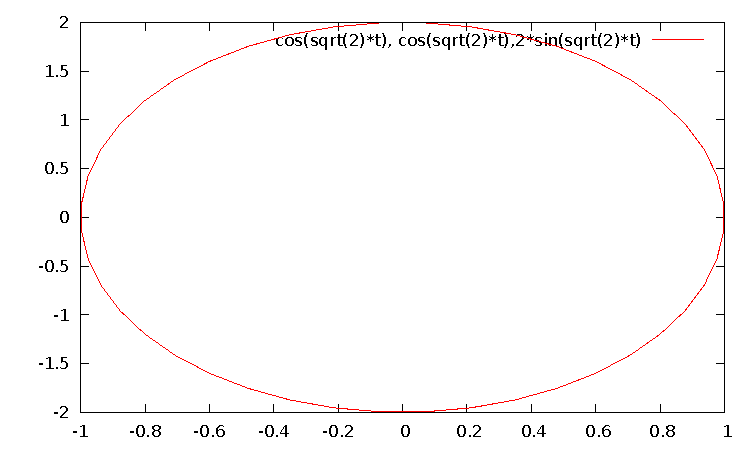
\includegraphics[width=\textwidth]{bahnkurve4c.pdf}}
\aufgabe{5}
\subsection*{a)}
\begin{description}
\item[Energie] bleibt erhalten, da keine Kräfte wirken.
\item[Impuls] bleibt erhalten, da keine Kräfte wirken.
\item[Drehimpuls bezüglich A] bleibt erhalten, da keine Kräfte wirken. $\vec L_A$ ist obendrein $\vec 0$, sofern $A$ auf der gestrichelten Linie liegt.
\item[Drehimpuls bezüglich B] bleibt erhalten, da keine Kräfte wirken.
\end{description}
\subsection*{b)}
\begin{description}
\item[Energie] bleibt erhalten, da $\vec F$ konservativ ist:
\begin{align}
\vec F(\vec r)&=f\left(\left|\vec r\right|\right)\cdot\vec e_r\\
\vec\nabla\times\vec F\left(\vec r\right)&=\vec 0
\end{align}
Letzteres folgt daraus, dass $f$ bloß von $\left|\vec r\right|$ abhängt.
\item[Impuls] bleibt nicht erhalten, da Kräfte wirken ($\vec F=\dot\vec p\neq\vec 0$).
\item[Drehimpuls bezüglich A] bleibt nicht erhalten, da $\frac{\diff\vec L}{\diff t}=\vec M=\vec x\times\vec F$ nicht verschwindet ($\vec F$ ist unabhängig von $\vec x$).
\item[Drehimpuls bezüglich B] bleibt erhalten, da $\frac{\diff\vec L}{\diff t}=\vec M=\vec x\times\vec F=\vec 0$, da $\vec x$ und $\vec F$ per Definition kollinear sind.
\end{description}
\end{document}
